\documentclass[UTF8]{article}
\usepackage[a4paper,bindingoffset=0.2in,%
            left=2.54cm,right=2.54cm,top=3cm,bottom=3cm,%
            ]{geometry}
\usepackage{ctex}
\usepackage{graphicx}
\usepackage{subfigure}
\usepackage{ulem}
\usepackage{float}
\usepackage{enumitem}
\usepackage{amsmath}
\usepackage{bm}
\usepackage{cite}
\usepackage{url}
\usepackage{pdfpages}
\usepackage{braket}
\usepackage{listings}
\usepackage{hyperref}
\setlist{labelindent=\parindent}
\setlist{noitemsep,labelindent=\parindent}
\setlist[enumerate]{label=\textbf{\arabic*}}
\renewcommand{\thefootnote}{\fnsymbol{footnote}} 

\hypersetup{
    	colorlinks = true, 
		linkcolor = black,
		citecolor = black,
		urlcolor = black
}

\lstset{
    basicstyle=\ttfamily,
    keywordstyle=\color{blue}\ttfamily,
    stringstyle=\color{red}\ttfamily,
    commentstyle=\it\color[RGB]{0,96,96},
    morecomment=[l][\color{magenta}]{\#},
    showstringspaces=false,                              % 不显示字符串中的空格
    numbers=left,                                        % 在左侧显示行号
	numberstyle=\tiny\color{gray},                       % 设定行号格式
	breaklines=true,
	rulesepcolor= \color{gray}, %代码块边框颜
	backgroundcolor=\color[RGB]{245,245,245},
	%backgroundcolor=\color{lightgray},
	frame=shadowbox%用方框框住代码块
}

\title{\bfseries 数字信号处理期末项目报告}
\author{林士翰~~15307130120\\院系:计算机科学技术学院\\专业:计算机科学与技术}
\begin{document}
\begin{titlepage}
	\maketitle
	\tableofcontents
	\thispagestyle{empty}
\end{titlepage}

\section{引言}
从上世纪60年代起至今,语音识别技术经历了漫长的发展过程。早期语音识别采用基于矢量量化(VQ)、动态时间归整(DTW)等的模版匹配方法,这类方法对小词汇量的孤立语音识别效果较好,但无法处理更复杂的识别任务\cite{lizhao2016speech}。20世纪80年代,隐马尔科夫模型(HMM)被引入语音识别任务中,其对语音信号时变过程的建模取得了很好的效果,成为语音识别技术发展的里程碑\cite{rabiner1989tutorial}。此外,Davis和Mermelstein提出了梅尔频率倒谱系数(MFCC),成为最重要的语音特征\cite{davis1980comparison}。此外,为了识别连续语音,语言模型被引入语音识别中,即从语料库中提取语言表达习惯,从而辅助连续词汇的识别。自此,提取MFCC特征并采用基于HMM和语言模型的识别算法成为1990年至2010年这20年之间最重要、最流行的语音识别框架,语音识别技术没有重大突破\cite{yunwang2018history}。2010年后,随着深度学习技术的迅速发展,语音识别引入神经网络后取得巨大进步,DNN-HMM、RNN-CTC等新的识别方法取得了较高的准确率。2017年,Google宣布其人工智能系统的语音识别准确率已经高达95\%\cite{fortune2017google}。语音识别技术经过半世纪的发展,终于使机器具有与人类相当的识别水平。

本项目中,我采用了三种识别算法实现孤立词的语音识别,包括动态时间归整(DTW)、混合高斯的隐马尔可夫模型(GMM-HMM)、卷积神经网络(CNN)。实验结果表明,传统方法,先提取语音信号特征(MFCC、LPC等),再使用DTW或GMM-HMM等模型进行训练和识别,准确率较低(<65\%),但采用了CNN后,无需人工筛选语音信号特征即可得到较高的准确率(>80\%),神经网络极大地提升了语音识别技术。

\section{识别算法}
本项目中我使用了DTW、GMM-HMM、CNN三种方法进行语音识别。

DTW和GMM-HMM为传统方法,在使用模型前需要从语音信号进行中提取特征,过程为:预加重、分帧、加窗、端点检测、特征提取。这样就得到语音段每一帧的特征向量,设语音段帧数为$P$,特征数为$M$,则每一遍录音都将得到一个$P \times M$的帧特征矩阵。最后用$N$个样本(录音)的特征矩阵训练模型。在进行测试时,需要先对测试的录音进行如上的特征提取操作,再使用模型得到判定结果。

传统方法进行复杂的特征提取过程的目的是为了弥补传统模型较弱的拟合能力。神经网络方法不但有强大的拟合能力,还能自动进行特征提取的过程,而且这些特征比人工筛选的特征更具有代表性,因为神经网络充分利用了数据的原始信息。我们可以省去特征提取的过程,在端点检测后即可将语音段直接输入模型进行训练或识别。

本节接下来简要介绍本项目中用到的预处理、端点检测、MFCC、LPC、DTW、GMM-HMM、CNN的原理和实现。本项目中,DTW相关的代码使用C++编写,其他代码使用Python编写。

\subsection{预处理}
预加重:实际录音得到的信号由于电流的``趋肤效应''导致高频成分比低频成分衰减严重,为了对高频成分进行补偿,增大信噪比,可以对信号进行预加重。一般使用高通滤波器$H(z)=1-\alpha z^{-1}$实现预加重,其中$\alpha$为预加重系数,在0.9到1.0之间,本项目中我选取0.95作为$\alpha$。将传递函数$H(z)$写为时域差分形式即为$y(n)=x(n)-\alpha x(n-1)$。对于一段录音,我们有完整的信号数据,可以简单使用时域差分形式实现预加重操作。

分帧加窗:人发音时声道的各个特征是随时间变化的,但是一段较小的时间内(<30ms)可以认为声道特征是不变的,因此可以将信号划分许多重叠的帧,提取每一帧的特征。本项目中,我选取20ms作为帧长,重叠为10ms,使用汉明窗$w(n)=\bigg[ 0.54-0.46 \cos(\frac{2\pi n}{N-1})\bigg]R_N(n)$对每一帧加窗。

\subsection{端点检测}
由于一段孤立词录音中不是时刻有语音的,删除无声段、噪音段,识别出真正的语音段不但可以加速特征提取和模型训练,还能减少噪声的干扰,提升准确率。我采用短时平均幅度E和过零率Z检测语音段端点。设$s_w(n)$为加窗后的信号,E和Z采用如下定义:
\begin{align*}
	E & =\sum_n |s_w(n)|                               \\ 
	Z & =\frac{1}{2}\sum_n |sgn(s_w(n))-sgn(s_w(n-1))| 
\end{align*}

我设置了四个阈值,最小幅度阈值MEH,过零率低阈值MZL,过零率高阈值MZH。经过多次尝试,我设计了如下三步端点检测方案:

\begin{figure}[t]
	\begin{center}
		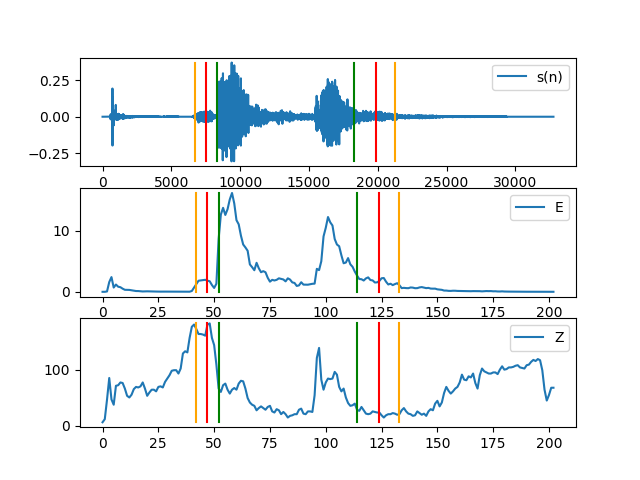
\includegraphics[width=\textwidth]{img/16307110258-11-15.png}
	\end{center}
	\caption{端点检测结果}
	\label{fig:epd}
\end{figure}

\begin{enumerate}
	\item 分别从左到右和从右到左找到第一个短时平均幅度大于MEH的帧,作为大致起点和终点,记为s1和e1。
	\item 从s1开始向前扫描,统计每5个帧短时平均幅度的平均值,如果下一个5个帧的平均值大于当前5个帧的平均值,则停止扫描,将这5个帧的开头帧记为s2。同理,从e1向后扫描获得e2。由于发音时能量往往先增大再减小,上述步骤可以找到第一个能量增长点和最后一个能量下降点,从而找到更准确的端点。使用平均值的原因是为了防止轻微的能量下降导致扫描中断。经过尝试,我限制s2(或e2)最多只能从s1(或e1)出发向前扫描3次,即$3 \times 5=15$帧。
	\item 清音过零率较高,浊音过零率较低,噪音居于两者之间,因此过大或过小的过零率都表明了一段语音。我从s2出发向前扫描,统计每8个帧的过零率的平均值,若平均值大于MZH或者小于MZL就继续向前扫描,直至发现过零率处于MZL到MZH之间,取开头帧为s3。同理可得e3。同样地,限制s3最多只能从s2出发向前扫描3次,但允许e3向后扫描5次,因为有些词语可能有较长的尾音。此外,当发现短时平均幅度小于MEL时,则停止扫描,因为可能碰到接近完全无声段,过零率也非常低。
\end{enumerate}

经过以上三步,s3到e3之间即为识别出得语音段。要获得较高的准确率就需要合理设置ME、MZL、MZH的值。经过尝试,我按照如下方式设置阈值:
\begin{enumerate}
	\item MEH为短时平均幅度最大值的0.15倍,MEL为最大值的0.05倍
	\item 由于录音开始后人的反应时间一般大于0.2秒,我选取前15帧当作噪声,统计它们过零率的平均值$NZ_{AVE}$和方差$NZ_{STD}$。根据高斯分布的$3\sigma$原则,令$MZL=NZ_{AVE}-3NZ_{STD},~~MZH=NZ_{AVE}+3NZ_{STD}$。
	\item 需要处理一些特殊情况:$NZ_{STD}$可能为0,导致MZL和MZH相等,无法拓展起点终点,这种情况下我令$NZ_{STD}=0.2NZ_{AVE}$;前15帧可能为几乎完全无声,导致$NZ_{AVE}$接近于0,这种情况下我让$NZ_{AVE}$等于最大过零率的0.5倍;前15帧的噪声可能导致$NZ_{AVE}$非常大,这种情况下我让$NZ_{AVE}$等于最大过零率的0.7倍。
\end{enumerate}

图~\ref{fig:epd}展示了三步法确定端点的过程,用绿、红、橙分别表示(s1, e1)、(s2, e2)、(s3, e3),可以发现检测结果较为准确。此外,我手动检测了约四分之一的数据集检测结果,发现结果都较为准确。

\subsection{MFCC}
梅尔倒谱系数(MFCC)是在Mel频率提取出来的特征。Mel频率能够较好地反应人的听觉特性,Mel频率与频率的转化如下:
\begin{align*}
	Mel(f)      & =2595 \times \lg (1+\frac{f}{700})  \\
	Mel^{-1}(m) & =700 \times (10^{\frac{m}{2595}}-1) 
\end{align*}

在Mel频率上等间隔划分出L个三角滤波器(本项目中L=26),对$s_w(n)$计算FFT,对频谱能量使用滤波器并提取离散余弦变换(DCT)的前M项系数(本项目中M=13),即得到MFCC。

MFCC只反应了一帧的特征,但是帧之间的变化也是很重要的,因此可以对MFCC求一阶差分和二阶差分,与MFCC结合组成$3 \times M$维度的特征向量。设$\bm{c}_k$为第k帧的M项MFCC构成的特征向量,根据\cite{huang2001spoken},我在本项目中将一阶差分$\bm{d}^{(1)}_k$和二阶差分$\bm{d}^{(2)}_k$定义为:
\begin{align*}
	\bm{d}^{(1)}_k & =\bm{c}_{k+2}-\bm{c}_{k-2}             \\
	\bm{d}^{(2)}_k & =\bm{d}^{(1)}_{k+1}-\bm{d}^{(1)}_{k-1} \\
\end{align*}

本项目中,我用Python实现了MFCC的过程,算法伪代码如下:
~\\
\lstinputlisting[]{code/mfcc.txt}
\vspace{10pt}

求一阶差分和二阶差分代码较简单,这里省略。

\subsection{LPC}
线性预测(LPC)用线性差分对语音信号进行建模,信号$s_w(n)$的预测值$\hat{s_w}(n)$由过去$p$个信号值线性组合得到,即
\[
	\hat{s_w}(n)=\sum_{i=1}^p a_i s_w(n-i)
\]

只要求出使预测误差$E=\sum_n e^2(n)=(s_w(n)-\hat{s_w}(n))^2$最小的$a$值,即可将$a_1, a_2, ..., a_p$作为语音信号的特征。经过推导,所求$a$值可以由以下线性方程组解出:
\begin{align*}
	   &\sum_{i=1}^p R(|k-i|)a_i=R(k), &k=1,2, ..., p        \\
	   &R(j)=\sum_{n=j}^{N-1} s_w(n)s_w(n-j), &j=1,2, ..., p 
\end{align*}

本项目中我直接使用高斯消元法求$a_i$,代码较简单,这里省略。我将LPC作为特征用在DTW和GMM-HMM模型中,但是发现它会导致识别准确率降低,应该是由于LPC对语音信号的刻画不够准确,导致对识别造成干扰。因此我最后没有将LPC应用到语音识别任务中。

\subsection{DTW}
DTW算法采用动态规划求解两个不同长度序列的最小距离。以下先介绍序列的最小距离问题。

设有两个序列$x(n),y(m), 1 \le n \le N, 1 \le m \le M \le N$。定义$x(i)$和$y(j)$之间的距离为$d(x(i), y(j))$。定义一个合法的匹配为$f: \{ 1, 2 .. N \} \mapsto \{ 1,2 .. M \} $,$f(i)$表示$x(i)$和$y(f(i))$对应,并且要求:(1) 对于${\forall} i_1 \le i_2, f(i_1) \le f(i_2)$; (2) $f(1)=1, f(N)=M$。定义序列$x$和$y$最小距离为$D=\sum_{i=1}^N d(x(i),y(f(i)))$,求$D_{min}$。

DTW算法思想如下:设$g(i,j)$表示$x(1..i)$与$y(1..j)$匹配所能得到的最小距离,则显然$g(i,j)=min\{g(i-1, j), g(i, j-1), g(i-1, j-1)\}+d(x(i), y(j))$,最后$D_{min}=g(N, M)$。

语音识别任务中,两段录音经过端点检测后获得语音信号长度往往不同,并且每个语音信号的特征由多个有序帧的特征向量组成。设$x(i)$和$y(i)$分别表示$x$和$y$的第$i$帧和第$j$帧,$x(i)$和$y(i)$均为$P$维向量,可定义$d(x(i), y(j))=\sqrt{\sum_{p}^P(x(i)_p-y(j)_p)^2}$。这样,我们就可以用DTW求出两段语音的距离,表征它们的相似程度,本节接下来的部分把这个距离称为DTW距离,用$DTW(x,y)$表示。

使用DTW算法训练语音识别模型的具体过程如下:
\begin{enumerate}
	\item 需要对每个单词建立一个模型。
	\item 对于每个单词,使用k-means对该单词所有录音进行聚类。在k-means中使用样本$x$和$y$的DTW距离表示他们距离$\delta(x, y)$。
	\item 对于每个类,用该类的``中心''来代表这个类。由于样本之间的距离使用DTW距离,需要重新定义类的``中心''。设某个类的包含的样本是$z_1, z_2, ..., z_q$,则中心定义为使得$\sum_{i=1}^qDTW(z_j,z_i)$最小的$z_j, 1 \le j \le p$。
	\item 对于每个单词,k-means聚类后的K个中心即是对应的模型。
\end{enumerate}

DTW识别的具体过程如下:
\begin{enumerate}
	\item 对于测试录音,计算他与每个单词的所有类中心的DTW距离。
	\item 与测试录音DTW距离最小的类中心所对应的单词即为判定词。
\end{enumerate}

DTW运算量巨大,使用Python实现无法应对大量数据,因此本项目中我用C++实现DTW和k-means,运算速度比用Python实现提升了20倍以上。DTW算法伪代码如下:
~\\
\lstinputlisting[]{code/dtw.txt}
\vspace{10pt}

K-means算法伪代码如下:
~\\
\lstinputlisting[]{code/kmeans.txt}

\subsection{GMM-HMM}
声道特征在一帧之内可以认为是不变的,但是在不同帧之间是变化的,而DTW和SVM等模型无法拟合这种时间上的变化,但是HMM却可以将时间上的变化用状态变化表示出来,所以HMM是语音建模的利器。声道特征随着人发出不同音素变化,HMM将音素变化看成状态的变化,在每个状态,以发射概率输出相应的观测值。朴素HMM每个状态观测值的发射概率由发射矩阵决定,但是GMM-HMM将GMM融合进HMM中,以表示状态的发射概率。GMM随着高斯分布个数增加可以拟合所有连续函数,可以用GMM计算每个状态每个观测值的发射概率。

GMM-HMM具体的模型训练过程如下:
\begin{enumerate}
	\item 需要对每个单词建立一个GMM-HMM模型。
	\item 对于一个单词的一遍录音,提取每一帧的特征向量,形成特征矩阵。
	\item 设每一帧的特征向量有M维,总共P帧。将P帧看成HMM的一个长度为P的观测序列$O_1O_2 ... O_P$,每个观测值$O_i$为一个M维特征向量,因此GMM需使用M维高斯分布。
	\item 将观测序列$O_1O_2 ... O_P$输入GMM-HMM中用EM算法同时训练GMM和HMM。
\end{enumerate}

GMM-HMM识别的具体过程如下:
\begin{enumerate}
	\item 提取测试录音每一帧的特征向量,得到观测序列。
	\item 用每个单词模型,用Viterbi求出该观测序列的最大生成概率,作为每个模型的得分。
	\item 得分最高的模型对应的单词即为判定词。
\end{enumerate}

本项目中,我直接调用hmmlearn库实现GMM-HMM,HMM状态数和每个状态的GMM分布数都设为5。

\subsection{CNN}
CNN在计算机视觉领域应用广泛,本项目中我把它用在语音识别上,取得了很好的效果。

全连接神经网络输出层每个神经元都由每个输入加权得到,这就导致巨大的参数数量和巨大的计算量。CNN采用卷积核让每个输出取决于一小部分的输入,这部分输入称为该输出的``感受野''。由于卷积核在所有输出之间共享,所以CNN具有``权值共享''的特点。这就大大减少了计算量,并且通过多层CNN叠加依然可以获得很好的识别效果。

一般来说,卷积核是个矩阵,若输入数据有n个通道(channel),则每个卷积核也有n个通道,每个卷积核的输出由n个通道的结果求和得到。所以卷积核的通道数取决于输入的通道数。CNN通常会采用多个卷积核,所以输出将有多个通道,通道数等于卷积核数目。

CNN其实相当于一个特征提取器,所以可以不进行MFCC等特征提取操作,直接将原始数据输入。CNN的输出结果还不能用于分类,因此一般在CNN后面叠加一层全连接网络,用softmax将输出映射为各个类别的概率,概率最高类别的即为判定结果。

\begin{figure}[H]
	\centering
	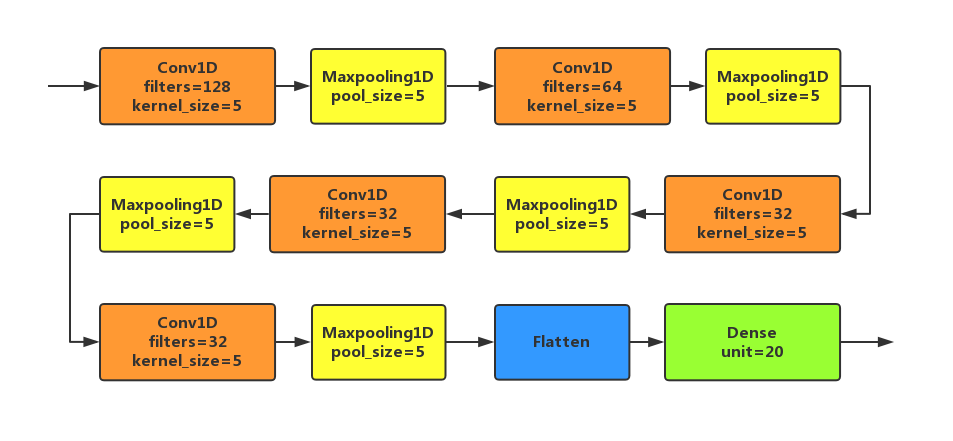
\includegraphics[width=\textwidth, trim=50 50 50 25, clip]{img/CNN.png}
	\caption{神经网络模型}
	\label{fig:CNN}
\end{figure}

本项目中,我使用了Keras库实现了五层CNN叠加,两层CNN中间加入maxpooling,最后一层flatten后连接到全连接网络进行判定,如图~\ref{fig:CNN}所示。语音识别的输入是一维音频,所以卷积核是一维形式。卷积核数量分别设为128、64、32、32、32,步长都为1。本项目数据只有一个通道,所以第一层CNN的卷积核是一个通道,接下来四层的卷积核通道数取决前一层的卷积核数量。

\section{实验方法}
本项目的数据集来自34个同学对20个单词的录音,每个同学每个单词有20次录音。在实验过程中,我发现有一位同学的录音质量较差,体现在背景噪音较大、录音未包含完整单词、录音标签与单词不匹配等,因此我将该同学的录音从数据集中删除,最后使用的数据集大小为$33 \times 20 \times 20=13200$。

我对模型的测试方法分为集内测试和集外测试。集内测试时,我先用整个数据集对模型进行训练,然后随机抽取数据集的10\%作为验证集,检验模型的准确率。集外测试时,我先随机选择3个同学,将他们所有的录音从数据集中剥离,作为验证集,剩下的数据集作为训练集对模型进行训练,最后用验证集检验模型准确率。两种测试方法的区别在于,集内测试的训练集中包含了验证集,而集外测试的验证集的同学录音完全不出现在训练集中,所以集内测试的准确率通常高于集外测试,但集外测试的结果体现了模型的泛化性,比较可靠。

除了准确率,我测量了三种方法的运行时间,分别考虑了他们的模型训练时间和识别时间。需要指出的是,DTW的计算量巨大,使用Python编写的脚本完成训练所需时间过长,所以我用C++实现了DTW相关代码,效率提升了20倍以上,而其他识别方法使用Python编写。本文不对Python与C++的效率进行换算,仅给出原始运行时间,所以比较时存在一定不公平性。运行时间测量采用的计算机配置如表~\ref{tab:machine}所示,不使用显卡。

\begin{table}[htbp]
	\centering
	\begin{tabular}{|c|c|c|}
		\hline
		\textbf{操作系统} & \textbf{CPU}                 & \textbf{内存} \\
		\hline
		macOS Mojave 10.14.4  & Intel Core i7 6700HQ 2.6 GHz & 16GB            \\
		\hline
	\end{tabular}
	\caption{\label{tab:machine}机器配置}
\end{table}

\section{实验结果}
表~\ref{tab:results}展示了三种方法在集内测试和集外测试的识别准确率,以及模型训练时间和识别时间。

\begin{table}[htbp]
	\centering
	\begin{tabular}{|l|c|c|c|c|c|}
		\hline
		                 & \textbf{编程语言} & \textbf{集内测试} & \textbf{集外测试} & \textbf{训练时间} & \textbf{识别时间} \\
		\hline
		\textbf{DTW}     & C++                   & 65.08\%               & 63.67\%               & 148s                  & 0.165s                \\
		\hline
		\textbf{GMM-HMM} & Python                & 14.92\%               & 10.58\%               & 270s                  & 0.026s                \\
		\hline
		\textbf{CNN}     & Python                & 90.70\%               & 82.67\%               & >4000s                & 0.009s                \\
		\hline
	\end{tabular}
	\caption{\label{tab:results}识别准确率与运行时间}
\end{table}

对比三种方法的准确率可以发现,GMM-HMM模型较复杂,但效果并不理想;DTW算法简单效果却比GMM-HMM好得多,具有一定的使用价值;神经网络相比传统方法确实有巨大优势,使用CNN不但省去了特征提取的过程,还获得高达90\%的准确率。

对比同一方法集内测试和集外测试结果可以发现,集内测试的准确率都比集外略高,这是由于集内测试时训练集已经包含了验证集的数据,不受过拟合的影响;而集外测试时,验证集说话人的录音则完全没有出现在训练集中,对模型的泛化性提出了更高的要求。

对比三种方法的运行时间可以发现,即使使用C++代替Python提升效率后,DTW仍然需要一定的训练时间,而且识别时间依然是三者中耗时最长的;GMM-HMM的训练时间和识别时间都位于中间;CNN需要大量的时间进行模型训练,但却只需要不到0.1秒的时间就可以进行识别,这也是很多神经网络的特点,高识别速度和高准确率使其可以用在实时识别当中。

\section{总结}
本项目是一个少量词汇的孤立词识别,我采用了两种传统方法——DTW与GMM-HMM,和较新的神经网络方法——CNN,实现识别系统,并对系统的准确率和计算速度两方面的性能进行测试。结果表明,GMM-HMM的准确率很不理想;DTW的准确率较高,但训练模型和识别都比较耗时;CNN方法拥有最高的准确率、最低的识别延迟,但是也需要最长的训练时间。本项目中我编写的核心代码包括:预处理、端点检测、MFCC、LPC、DTW、k-means,其他代码主要调用了wave、hmmlearn、Keras这些库。项目代码已上传至\url{https://github.com/SHiftLin/DSP_Project}。

\bibliography{ref}
\bibliographystyle{abbrv}

\end{document}
